\documentclass[tikz,border=0pt]{standalone}
% Estilo común de figuras y animaciones (mismos colores que la presentación)
% Compilar con XeLaTeX o LuaLaTeX (fuente TeX Gyre Heros); con pdfLaTeX usa Latin Modern Sans.
\usepackage{iftex}
\ifPDFTeX
  \usepackage[utf8]{inputenc}\usepackage[T1]{fontenc}\usepackage{lmodern}
  \renewcommand{\familydefault}{\sfdefault}
\else
  \usepackage{fontspec}\setmainfont{TeX Gyre Heros}\setsansfont{TeX Gyre Heros}
\fi
\usepackage{amssymb}
\usetikzlibrary{arrows.meta,positioning,calc,shapes.geometric,shadows,decorations.pathreplacing}
\definecolor{azul}{HTML}{1F3A5F}
\definecolor{acento}{HTML}{C0392B}
\definecolor{suave}{HTML}{EEF2F7}
\definecolor{gris}{HTML}{6B7280}
\definecolor{cOur}{HTML}{D62728}
\definecolor{cLib}{HTML}{1F77B4}
\definecolor{cWil}{HTML}{2CA02C}
\definecolor{cFol}{HTML}{FF7F0E}
\definecolor{cAnd}{HTML}{9467BD}
\definecolor{amarillo}{HTML}{F6C343}
\definecolor{verde}{HTML}{2E8B57}

% ---------- Iconos ----------
\providecommand{\iconscale}{1}
% \robot{pos}{color}{nombre}
\newcommand{\robot}[3]{%
  \begin{scope}[shift={#1}, scale=\iconscale, transform shape]
    \draw[#2, line width=0.8pt] (0,0.62) -- (0,0.78); \fill[#2] (0,0.8) circle (0.05);
    \draw[fill=#2!15, draw=#2, line width=0.8pt, rounded corners=2pt] (-0.3,0.25) rectangle (0.3,0.62);
    \fill[#2] (-0.13,0.45) circle (0.05); \fill[#2] (0.13,0.45) circle (0.05);
    \draw[#2, line width=0.6pt] (-0.1,0.33) -- (0.1,0.33);
    \draw[fill=#2!25, draw=#2, line width=0.8pt, rounded corners=2pt] (-0.24,-0.2) rectangle (0.24,0.22);
    \node[font=\tiny\bfseries, #2!70!black] at (0,-0.33) {#3};
  \end{scope}}
% \persona{pos}{color}{nombre}
\newcommand{\persona}[3]{%
  \begin{scope}[shift={#1}, scale=\iconscale, transform shape]
    \draw[fill=#2!20, draw=#2, line width=0.8pt] (0,0.5) circle (0.17);
    \draw[fill=#2!35, draw=#2, line width=0.8pt] (-0.27,-0.2) .. controls (-0.27,0.25) and (0.27,0.25) .. (0.27,-0.2) -- cycle;
    \node[font=\tiny\bfseries, #2!70!black] at (0,-0.33) {#3};
  \end{scope}}
% \libro{pos}{color}{texto}
\newcommand{\libro}[3]{%
  \begin{scope}[shift={#1}, scale=\iconscale, transform shape]
    \draw[fill=#2!25, draw=#2!80!black, line width=0.7pt, rounded corners=1pt] (-0.25,-0.32) rectangle (0.25,0.32);
    \fill[#2!80!black] (-0.25,-0.32) rectangle (-0.18,0.32);
    \node[font=\tiny\bfseries, align=center] at (0.035,0) {#3};
  \end{scope}}
% \letrero{pos}{texto principal}{tickets}
\newcommand{\letrero}[3]{%
  \begin{scope}[shift={#1}, scale=\iconscale, transform shape]
    \draw[fill=azul, draw=azul!60!black, rounded corners=2pt, line width=0.8pt] (-0.95,-0.32) rectangle (0.95,0.32);
    \foreach \i in {0,...,3} {\fill[cFol] (-0.85+\i*0.11,0.12) rectangle ++(0.08,0.12);}
    \foreach \i in {4,...,15} {\fill[amarillo!80] (-0.85+\i*0.11,0.12) rectangle ++(0.08,0.12);}
    \node[font=\tiny\bfseries, white] at (0,-0.12) {#2};
    \node[font=\tiny, cFol, anchor=south] at (-0.66,0.32) {#3};
  \end{scope}}
% \trituradora{pos}
\newcommand{\trituradora}[1]{%
  \begin{scope}[shift={#1}, scale=\iconscale, transform shape]
    \draw[fill=gris!25, draw=gris, line width=0.8pt] (-0.35,-0.25) rectangle (0.35,0.1);
    \draw[fill=gris!50, draw=gris] (-0.42,0.1) rectangle (0.42,0.2);
    \foreach \x in {-0.25,-0.12,0.01,0.14,0.27} {\draw[gris, line width=0.6pt] (\x,-0.25) -- (\x-0.03,-0.42);}
  \end{scope}}
% \ticket{pos}{color}
\newcommand{\ticket}[2]{%
  \begin{scope}[shift={#1}, scale=\iconscale, transform shape]
    \draw[fill=#2!30, draw=#2!80!black, line width=0.6pt] (-0.16,-0.09) -- (0.16,-0.09) -- (0.16,-0.03) arc (270:90:0.03) -- (0.16,0.09) -- (-0.16,0.09) -- (-0.16,0.03) arc (90:-90:0.03) -- cycle;
  \end{scope}}
% \contador{pos}{valor}{color}
\newcommand{\contador}[3]{%
  \node[scale=\iconscale, draw=#3, fill=white, line width=0.8pt, circle, inner sep=1.2pt, minimum size=0.42cm, font=\scriptsize\bfseries, text=#3] at #1 {#2};}

\renewcommand{\iconscale}{1.6}
\begin{document}
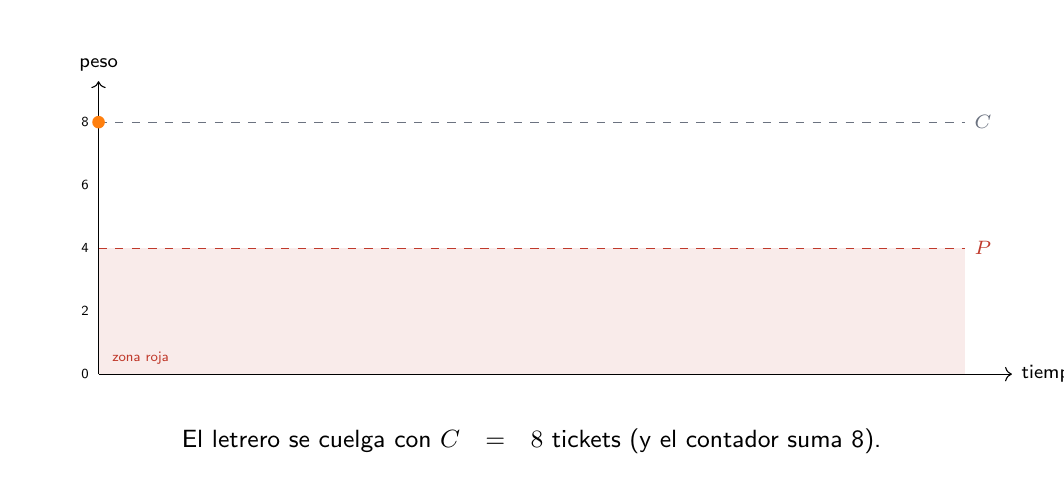
\begin{tikzpicture}
\useasboundingbox[fill=white] (0,0) rectangle (12.8,5.6);
\fill[acento!10] (0.9,1.2) rectangle (11.9,2.8);
\node[font=\tiny, acento, anchor=south west] at (0.95,1.2) {zona roja};
\draw[dashed, acento] (0.9,2.8) -- (11.9,2.8) node[right, font=\scriptsize] {$P$};
\draw[dashed, gris] (0.9,4.4) -- (11.9,4.4) node[right, font=\scriptsize] {$C$};
\draw[->] (0.9,1.2) -- (0.9,4.920000000000001) node[above, font=\scriptsize] {peso};
\draw[->] (0.9,1.2) -- (12.5,1.2) node[right, font=\scriptsize] {tiempo};
\node[left, font=\tiny] at (0.9,1.2) {0};
\node[left, font=\tiny] at (0.9,2.0) {2};
\node[left, font=\tiny] at (0.9,2.8) {4};
\node[left, font=\tiny] at (0.9,3.6000000000000005) {6};
\node[left, font=\tiny] at (0.9,4.4) {8};
\fill[cFol] (0.9,4.4) circle (0.08);
\node[font=\small, text width=12.2cm, align=center, text=black] at (6.4,0.35) {El letrero se cuelga con $C=8$ tickets (y el contador suma 8).};
\end{tikzpicture}

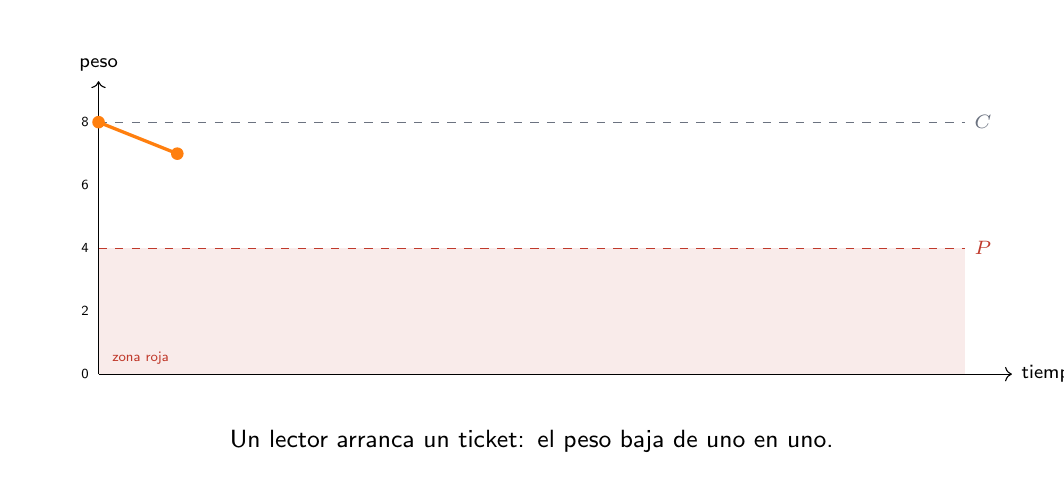
\begin{tikzpicture}
\useasboundingbox[fill=white] (0,0) rectangle (12.8,5.6);
\fill[acento!10] (0.9,1.2) rectangle (11.9,2.8);
\node[font=\tiny, acento, anchor=south west] at (0.95,1.2) {zona roja};
\draw[dashed, acento] (0.9,2.8) -- (11.9,2.8) node[right, font=\scriptsize] {$P$};
\draw[dashed, gris] (0.9,4.4) -- (11.9,4.4) node[right, font=\scriptsize] {$C$};
\draw[->] (0.9,1.2) -- (0.9,4.920000000000001) node[above, font=\scriptsize] {peso};
\draw[->] (0.9,1.2) -- (12.5,1.2) node[right, font=\scriptsize] {tiempo};
\node[left, font=\tiny] at (0.9,1.2) {0};
\node[left, font=\tiny] at (0.9,2.0) {2};
\node[left, font=\tiny] at (0.9,2.8) {4};
\node[left, font=\tiny] at (0.9,3.6000000000000005) {6};
\node[left, font=\tiny] at (0.9,4.4) {8};
\draw[very thick, cFol] (0.9,4.4) -- (1.9,4.0);
\fill[cFol] (0.9,4.4) circle (0.08);
\fill[cFol] (1.9,4.0) circle (0.08);
\node[font=\small, text width=12.2cm, align=center, text=black] at (6.4,0.35) {Un lector arranca un ticket: el peso baja de uno en uno.};
\end{tikzpicture}

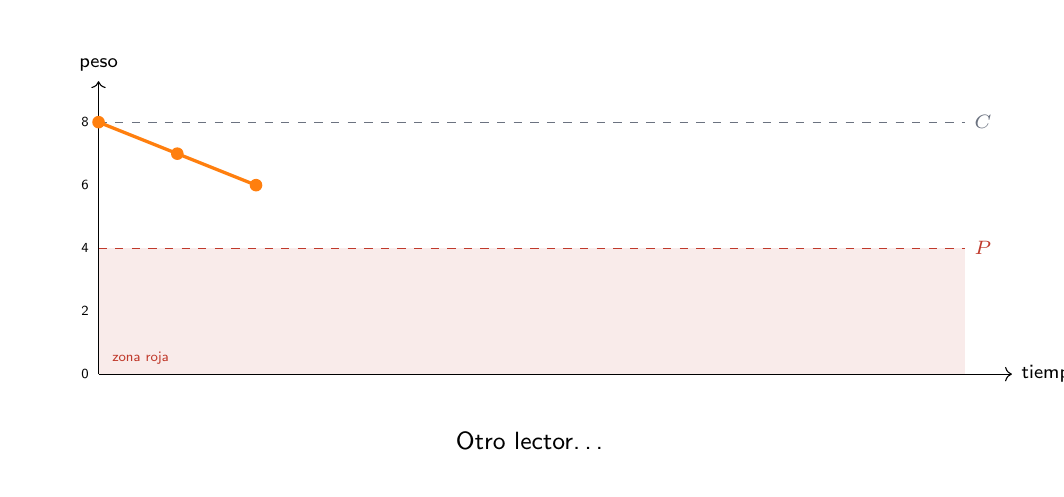
\begin{tikzpicture}
\useasboundingbox[fill=white] (0,0) rectangle (12.8,5.6);
\fill[acento!10] (0.9,1.2) rectangle (11.9,2.8);
\node[font=\tiny, acento, anchor=south west] at (0.95,1.2) {zona roja};
\draw[dashed, acento] (0.9,2.8) -- (11.9,2.8) node[right, font=\scriptsize] {$P$};
\draw[dashed, gris] (0.9,4.4) -- (11.9,4.4) node[right, font=\scriptsize] {$C$};
\draw[->] (0.9,1.2) -- (0.9,4.920000000000001) node[above, font=\scriptsize] {peso};
\draw[->] (0.9,1.2) -- (12.5,1.2) node[right, font=\scriptsize] {tiempo};
\node[left, font=\tiny] at (0.9,1.2) {0};
\node[left, font=\tiny] at (0.9,2.0) {2};
\node[left, font=\tiny] at (0.9,2.8) {4};
\node[left, font=\tiny] at (0.9,3.6000000000000005) {6};
\node[left, font=\tiny] at (0.9,4.4) {8};
\draw[very thick, cFol] (0.9,4.4) -- (1.9,4.0) -- (2.9,3.6000000000000005);
\fill[cFol] (0.9,4.4) circle (0.08);
\fill[cFol] (1.9,4.0) circle (0.08);
\fill[cFol] (2.9,3.6000000000000005) circle (0.08);
\node[font=\small, text width=12.2cm, align=center, text=black] at (6.4,0.35) {Otro lector\ldots};
\end{tikzpicture}

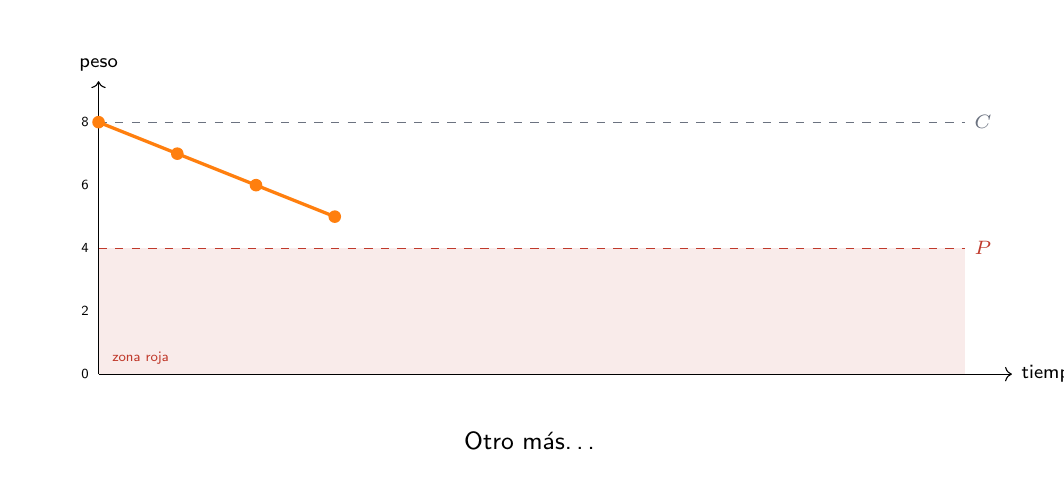
\begin{tikzpicture}
\useasboundingbox[fill=white] (0,0) rectangle (12.8,5.6);
\fill[acento!10] (0.9,1.2) rectangle (11.9,2.8);
\node[font=\tiny, acento, anchor=south west] at (0.95,1.2) {zona roja};
\draw[dashed, acento] (0.9,2.8) -- (11.9,2.8) node[right, font=\scriptsize] {$P$};
\draw[dashed, gris] (0.9,4.4) -- (11.9,4.4) node[right, font=\scriptsize] {$C$};
\draw[->] (0.9,1.2) -- (0.9,4.920000000000001) node[above, font=\scriptsize] {peso};
\draw[->] (0.9,1.2) -- (12.5,1.2) node[right, font=\scriptsize] {tiempo};
\node[left, font=\tiny] at (0.9,1.2) {0};
\node[left, font=\tiny] at (0.9,2.0) {2};
\node[left, font=\tiny] at (0.9,2.8) {4};
\node[left, font=\tiny] at (0.9,3.6000000000000005) {6};
\node[left, font=\tiny] at (0.9,4.4) {8};
\draw[very thick, cFol] (0.9,4.4) -- (1.9,4.0) -- (2.9,3.6000000000000005) -- (3.9,3.2);
\fill[cFol] (0.9,4.4) circle (0.08);
\fill[cFol] (1.9,4.0) circle (0.08);
\fill[cFol] (2.9,3.6000000000000005) circle (0.08);
\fill[cFol] (3.9,3.2) circle (0.08);
\node[font=\small, text width=12.2cm, align=center, text=black] at (6.4,0.35) {Otro más\ldots};
\end{tikzpicture}

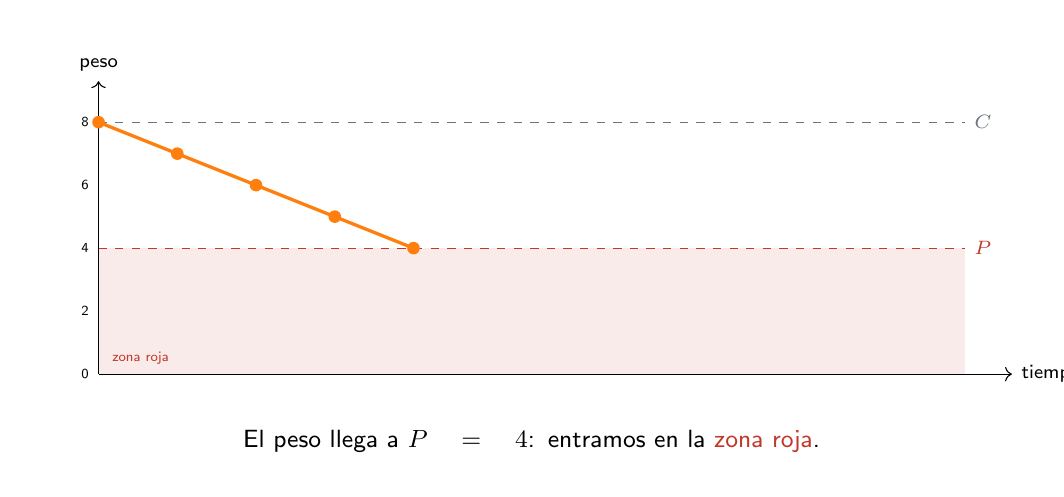
\begin{tikzpicture}
\useasboundingbox[fill=white] (0,0) rectangle (12.8,5.6);
\fill[acento!10] (0.9,1.2) rectangle (11.9,2.8);
\node[font=\tiny, acento, anchor=south west] at (0.95,1.2) {zona roja};
\draw[dashed, acento] (0.9,2.8) -- (11.9,2.8) node[right, font=\scriptsize] {$P$};
\draw[dashed, gris] (0.9,4.4) -- (11.9,4.4) node[right, font=\scriptsize] {$C$};
\draw[->] (0.9,1.2) -- (0.9,4.920000000000001) node[above, font=\scriptsize] {peso};
\draw[->] (0.9,1.2) -- (12.5,1.2) node[right, font=\scriptsize] {tiempo};
\node[left, font=\tiny] at (0.9,1.2) {0};
\node[left, font=\tiny] at (0.9,2.0) {2};
\node[left, font=\tiny] at (0.9,2.8) {4};
\node[left, font=\tiny] at (0.9,3.6000000000000005) {6};
\node[left, font=\tiny] at (0.9,4.4) {8};
\draw[very thick, cFol] (0.9,4.4) -- (1.9,4.0) -- (2.9,3.6000000000000005) -- (3.9,3.2) -- (4.9,2.8);
\fill[cFol] (0.9,4.4) circle (0.08);
\fill[cFol] (1.9,4.0) circle (0.08);
\fill[cFol] (2.9,3.6000000000000005) circle (0.08);
\fill[cFol] (3.9,3.2) circle (0.08);
\fill[cFol] (4.9,2.8) circle (0.08);
\node[font=\small, text width=12.2cm, align=center, text=black] at (6.4,0.35) {El peso llega a $P=4$: entramos en la \textcolor{acento}{zona roja}.};
\end{tikzpicture}

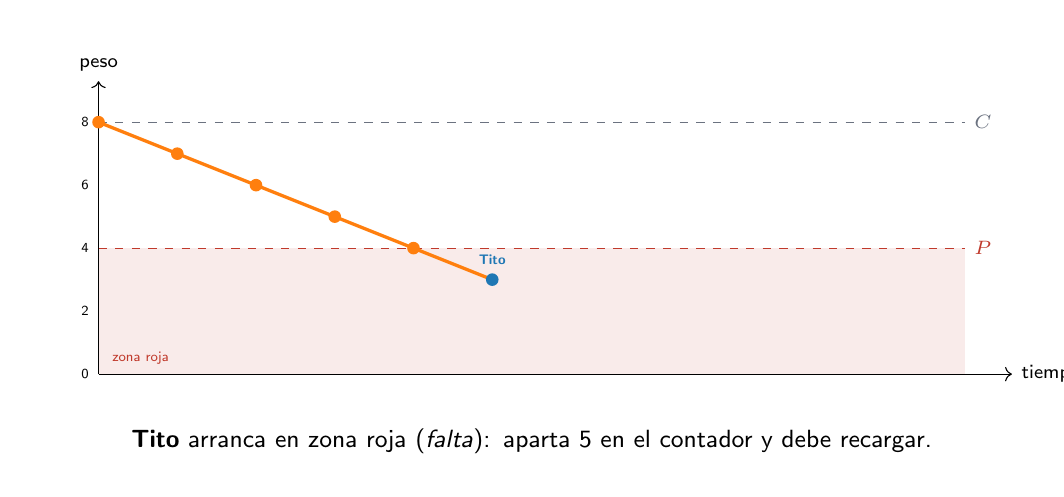
\begin{tikzpicture}
\useasboundingbox[fill=white] (0,0) rectangle (12.8,5.6);
\fill[acento!10] (0.9,1.2) rectangle (11.9,2.8);
\node[font=\tiny, acento, anchor=south west] at (0.95,1.2) {zona roja};
\draw[dashed, acento] (0.9,2.8) -- (11.9,2.8) node[right, font=\scriptsize] {$P$};
\draw[dashed, gris] (0.9,4.4) -- (11.9,4.4) node[right, font=\scriptsize] {$C$};
\draw[->] (0.9,1.2) -- (0.9,4.920000000000001) node[above, font=\scriptsize] {peso};
\draw[->] (0.9,1.2) -- (12.5,1.2) node[right, font=\scriptsize] {tiempo};
\node[left, font=\tiny] at (0.9,1.2) {0};
\node[left, font=\tiny] at (0.9,2.0) {2};
\node[left, font=\tiny] at (0.9,2.8) {4};
\node[left, font=\tiny] at (0.9,3.6000000000000005) {6};
\node[left, font=\tiny] at (0.9,4.4) {8};
\draw[very thick, cFol] (0.9,4.4) -- (1.9,4.0) -- (2.9,3.6000000000000005) -- (3.9,3.2) -- (4.9,2.8) -- (5.9,2.4000000000000004);
\fill[cFol] (0.9,4.4) circle (0.08);
\fill[cFol] (1.9,4.0) circle (0.08);
\fill[cFol] (2.9,3.6000000000000005) circle (0.08);
\fill[cFol] (3.9,3.2) circle (0.08);
\fill[cFol] (4.9,2.8) circle (0.08);
\fill[cLib] (5.9,2.4000000000000004) circle (0.08);
\node[font=\tiny\bfseries, text=cLib, above=2pt] at (5.9,2.4000000000000004) {Tito};
\node[font=\small, text width=12.2cm, align=center, text=black] at (6.4,0.35) {\textbf{Tito} arranca en zona roja (\emph{falta}): aparta 5 en el contador y debe recargar.};
\end{tikzpicture}

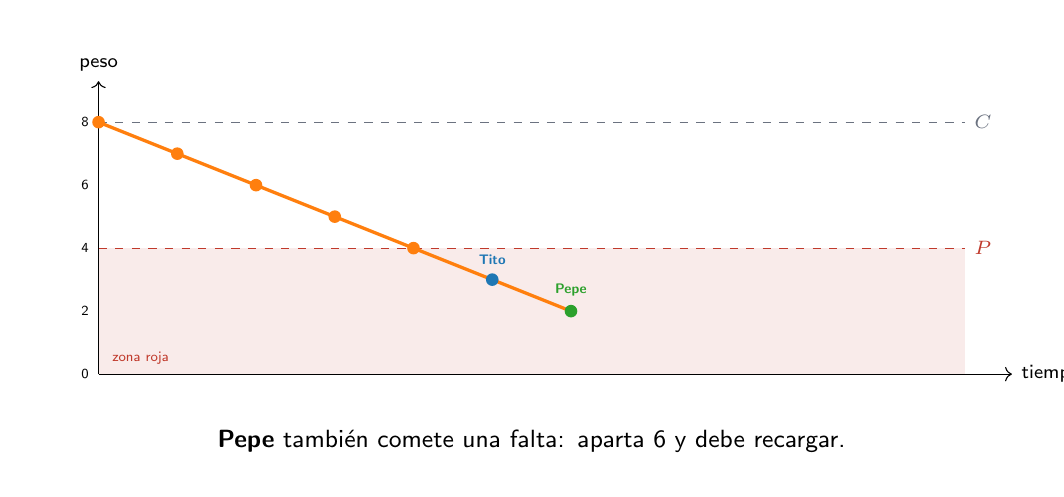
\begin{tikzpicture}
\useasboundingbox[fill=white] (0,0) rectangle (12.8,5.6);
\fill[acento!10] (0.9,1.2) rectangle (11.9,2.8);
\node[font=\tiny, acento, anchor=south west] at (0.95,1.2) {zona roja};
\draw[dashed, acento] (0.9,2.8) -- (11.9,2.8) node[right, font=\scriptsize] {$P$};
\draw[dashed, gris] (0.9,4.4) -- (11.9,4.4) node[right, font=\scriptsize] {$C$};
\draw[->] (0.9,1.2) -- (0.9,4.920000000000001) node[above, font=\scriptsize] {peso};
\draw[->] (0.9,1.2) -- (12.5,1.2) node[right, font=\scriptsize] {tiempo};
\node[left, font=\tiny] at (0.9,1.2) {0};
\node[left, font=\tiny] at (0.9,2.0) {2};
\node[left, font=\tiny] at (0.9,2.8) {4};
\node[left, font=\tiny] at (0.9,3.6000000000000005) {6};
\node[left, font=\tiny] at (0.9,4.4) {8};
\draw[very thick, cFol] (0.9,4.4) -- (1.9,4.0) -- (2.9,3.6000000000000005) -- (3.9,3.2) -- (4.9,2.8) -- (5.9,2.4000000000000004) -- (6.9,2.0);
\fill[cFol] (0.9,4.4) circle (0.08);
\fill[cFol] (1.9,4.0) circle (0.08);
\fill[cFol] (2.9,3.6000000000000005) circle (0.08);
\fill[cFol] (3.9,3.2) circle (0.08);
\fill[cFol] (4.9,2.8) circle (0.08);
\fill[cLib] (5.9,2.4000000000000004) circle (0.08);
\node[font=\tiny\bfseries, text=cLib, above=2pt] at (5.9,2.4000000000000004) {Tito};
\fill[cWil] (6.9,2.0) circle (0.08);
\node[font=\tiny\bfseries, text=cWil, above=2pt] at (6.9,2.0) {Pepe};
\node[font=\small, text width=12.2cm, align=center, text=black] at (6.4,0.35) {\textbf{Pepe} también comete una falta: aparta 6 y debe recargar.};
\end{tikzpicture}

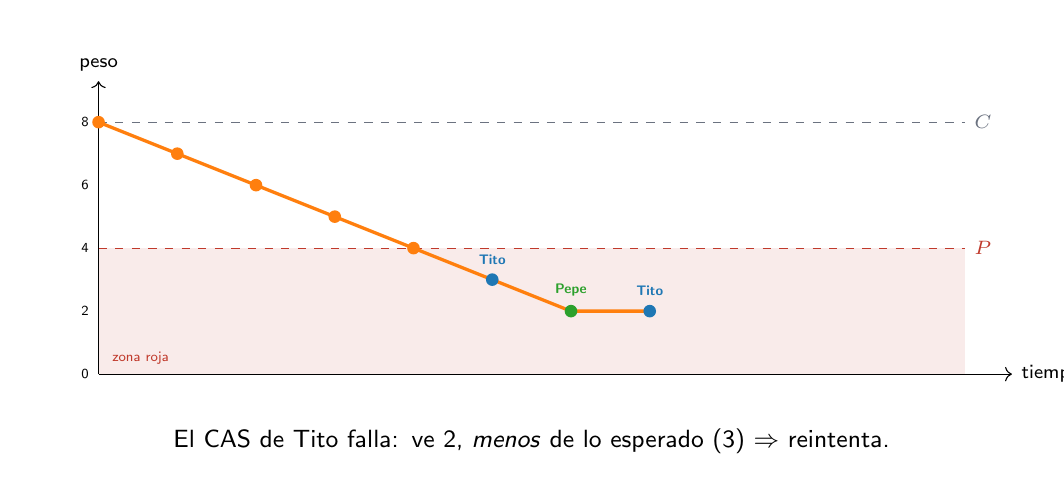
\begin{tikzpicture}
\useasboundingbox[fill=white] (0,0) rectangle (12.8,5.6);
\fill[acento!10] (0.9,1.2) rectangle (11.9,2.8);
\node[font=\tiny, acento, anchor=south west] at (0.95,1.2) {zona roja};
\draw[dashed, acento] (0.9,2.8) -- (11.9,2.8) node[right, font=\scriptsize] {$P$};
\draw[dashed, gris] (0.9,4.4) -- (11.9,4.4) node[right, font=\scriptsize] {$C$};
\draw[->] (0.9,1.2) -- (0.9,4.920000000000001) node[above, font=\scriptsize] {peso};
\draw[->] (0.9,1.2) -- (12.5,1.2) node[right, font=\scriptsize] {tiempo};
\node[left, font=\tiny] at (0.9,1.2) {0};
\node[left, font=\tiny] at (0.9,2.0) {2};
\node[left, font=\tiny] at (0.9,2.8) {4};
\node[left, font=\tiny] at (0.9,3.6000000000000005) {6};
\node[left, font=\tiny] at (0.9,4.4) {8};
\draw[very thick, cFol] (0.9,4.4) -- (1.9,4.0) -- (2.9,3.6000000000000005) -- (3.9,3.2) -- (4.9,2.8) -- (5.9,2.4000000000000004) -- (6.9,2.0) -- (7.9,2.0);
\fill[cFol] (0.9,4.4) circle (0.08);
\fill[cFol] (1.9,4.0) circle (0.08);
\fill[cFol] (2.9,3.6000000000000005) circle (0.08);
\fill[cFol] (3.9,3.2) circle (0.08);
\fill[cFol] (4.9,2.8) circle (0.08);
\fill[cLib] (5.9,2.4000000000000004) circle (0.08);
\node[font=\tiny\bfseries, text=cLib, above=2pt] at (5.9,2.4000000000000004) {Tito};
\fill[cWil] (6.9,2.0) circle (0.08);
\node[font=\tiny\bfseries, text=cWil, above=2pt] at (6.9,2.0) {Pepe};
\fill[cLib] (7.9,2.0) circle (0.08);
\node[font=\tiny\bfseries, text=cLib, above=2pt] at (7.9,2.0) {Tito};
\node[font=\small, text width=12.2cm, align=center, text=black] at (6.4,0.35) {El CAS de Tito falla: ve 2, \emph{menos} de lo esperado (3) $\Rightarrow$ reintenta.};
\end{tikzpicture}

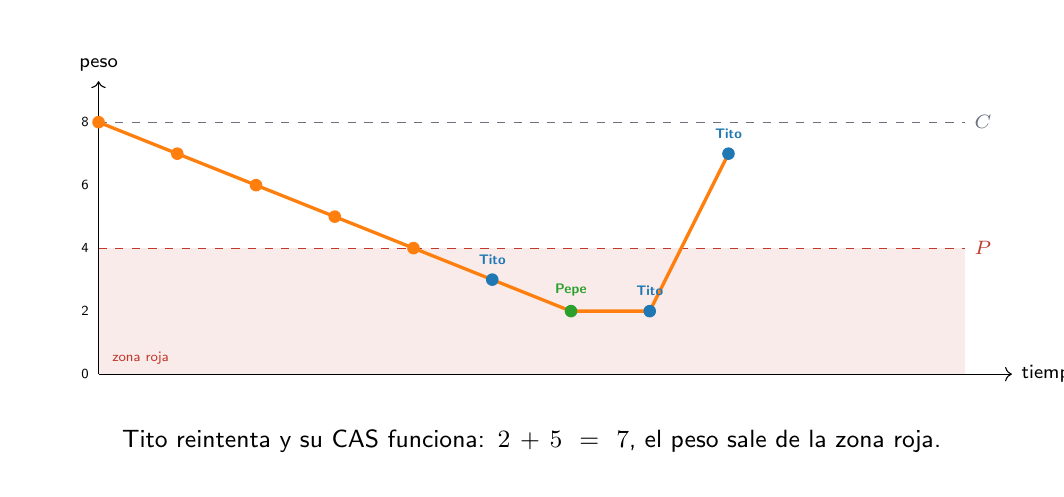
\begin{tikzpicture}
\useasboundingbox[fill=white] (0,0) rectangle (12.8,5.6);
\fill[acento!10] (0.9,1.2) rectangle (11.9,2.8);
\node[font=\tiny, acento, anchor=south west] at (0.95,1.2) {zona roja};
\draw[dashed, acento] (0.9,2.8) -- (11.9,2.8) node[right, font=\scriptsize] {$P$};
\draw[dashed, gris] (0.9,4.4) -- (11.9,4.4) node[right, font=\scriptsize] {$C$};
\draw[->] (0.9,1.2) -- (0.9,4.920000000000001) node[above, font=\scriptsize] {peso};
\draw[->] (0.9,1.2) -- (12.5,1.2) node[right, font=\scriptsize] {tiempo};
\node[left, font=\tiny] at (0.9,1.2) {0};
\node[left, font=\tiny] at (0.9,2.0) {2};
\node[left, font=\tiny] at (0.9,2.8) {4};
\node[left, font=\tiny] at (0.9,3.6000000000000005) {6};
\node[left, font=\tiny] at (0.9,4.4) {8};
\draw[very thick, cFol] (0.9,4.4) -- (1.9,4.0) -- (2.9,3.6000000000000005) -- (3.9,3.2) -- (4.9,2.8) -- (5.9,2.4000000000000004) -- (6.9,2.0) -- (7.9,2.0) -- (8.9,4.0);
\fill[cFol] (0.9,4.4) circle (0.08);
\fill[cFol] (1.9,4.0) circle (0.08);
\fill[cFol] (2.9,3.6000000000000005) circle (0.08);
\fill[cFol] (3.9,3.2) circle (0.08);
\fill[cFol] (4.9,2.8) circle (0.08);
\fill[cLib] (5.9,2.4000000000000004) circle (0.08);
\node[font=\tiny\bfseries, text=cLib, above=2pt] at (5.9,2.4000000000000004) {Tito};
\fill[cWil] (6.9,2.0) circle (0.08);
\node[font=\tiny\bfseries, text=cWil, above=2pt] at (6.9,2.0) {Pepe};
\fill[cLib] (7.9,2.0) circle (0.08);
\node[font=\tiny\bfseries, text=cLib, above=2pt] at (7.9,2.0) {Tito};
\fill[cLib] (8.9,4.0) circle (0.08);
\node[font=\tiny\bfseries, text=cLib, above=2pt] at (8.9,4.0) {Tito};
\node[font=\small, text width=12.2cm, align=center, text=black] at (6.4,0.35) {Tito reintenta y su CAS funciona: $2 + 5 = 7$, el peso sale de la zona roja.};
\end{tikzpicture}

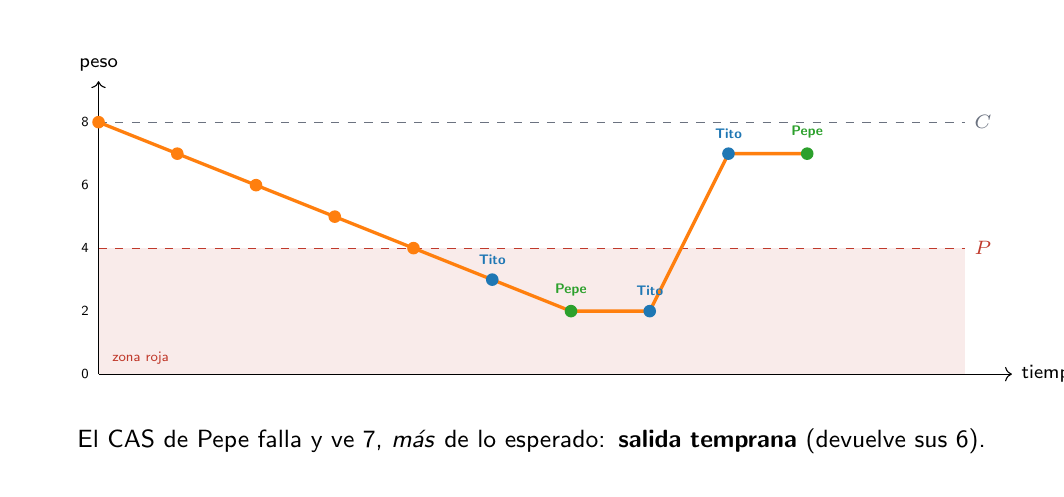
\begin{tikzpicture}
\useasboundingbox[fill=white] (0,0) rectangle (12.8,5.6);
\fill[acento!10] (0.9,1.2) rectangle (11.9,2.8);
\node[font=\tiny, acento, anchor=south west] at (0.95,1.2) {zona roja};
\draw[dashed, acento] (0.9,2.8) -- (11.9,2.8) node[right, font=\scriptsize] {$P$};
\draw[dashed, gris] (0.9,4.4) -- (11.9,4.4) node[right, font=\scriptsize] {$C$};
\draw[->] (0.9,1.2) -- (0.9,4.920000000000001) node[above, font=\scriptsize] {peso};
\draw[->] (0.9,1.2) -- (12.5,1.2) node[right, font=\scriptsize] {tiempo};
\node[left, font=\tiny] at (0.9,1.2) {0};
\node[left, font=\tiny] at (0.9,2.0) {2};
\node[left, font=\tiny] at (0.9,2.8) {4};
\node[left, font=\tiny] at (0.9,3.6000000000000005) {6};
\node[left, font=\tiny] at (0.9,4.4) {8};
\draw[very thick, cFol] (0.9,4.4) -- (1.9,4.0) -- (2.9,3.6000000000000005) -- (3.9,3.2) -- (4.9,2.8) -- (5.9,2.4000000000000004) -- (6.9,2.0) -- (7.9,2.0) -- (8.9,4.0) -- (9.9,4.0);
\fill[cFol] (0.9,4.4) circle (0.08);
\fill[cFol] (1.9,4.0) circle (0.08);
\fill[cFol] (2.9,3.6000000000000005) circle (0.08);
\fill[cFol] (3.9,3.2) circle (0.08);
\fill[cFol] (4.9,2.8) circle (0.08);
\fill[cLib] (5.9,2.4000000000000004) circle (0.08);
\node[font=\tiny\bfseries, text=cLib, above=2pt] at (5.9,2.4000000000000004) {Tito};
\fill[cWil] (6.9,2.0) circle (0.08);
\node[font=\tiny\bfseries, text=cWil, above=2pt] at (6.9,2.0) {Pepe};
\fill[cLib] (7.9,2.0) circle (0.08);
\node[font=\tiny\bfseries, text=cLib, above=2pt] at (7.9,2.0) {Tito};
\fill[cLib] (8.9,4.0) circle (0.08);
\node[font=\tiny\bfseries, text=cLib, above=2pt] at (8.9,4.0) {Tito};
\fill[cWil] (9.9,4.0) circle (0.08);
\node[font=\tiny\bfseries, text=cWil, above=2pt] at (9.9,4.0) {Pepe};
\node[font=\small, text width=12.2cm, align=center, text=black] at (6.4,0.35) {El CAS de Pepe falla y ve 7, \emph{más} de lo esperado: \textbf{salida temprana} (devuelve sus 6).};
\end{tikzpicture}

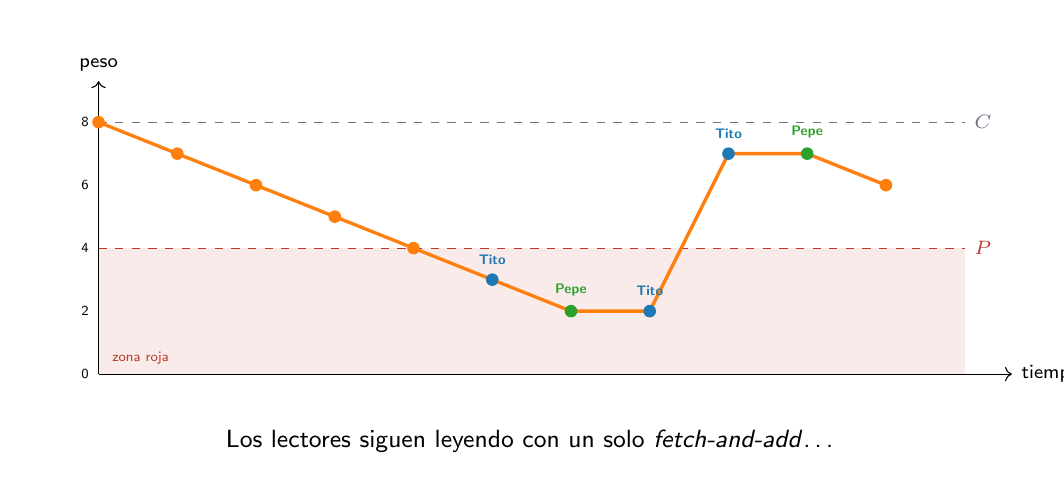
\begin{tikzpicture}
\useasboundingbox[fill=white] (0,0) rectangle (12.8,5.6);
\fill[acento!10] (0.9,1.2) rectangle (11.9,2.8);
\node[font=\tiny, acento, anchor=south west] at (0.95,1.2) {zona roja};
\draw[dashed, acento] (0.9,2.8) -- (11.9,2.8) node[right, font=\scriptsize] {$P$};
\draw[dashed, gris] (0.9,4.4) -- (11.9,4.4) node[right, font=\scriptsize] {$C$};
\draw[->] (0.9,1.2) -- (0.9,4.920000000000001) node[above, font=\scriptsize] {peso};
\draw[->] (0.9,1.2) -- (12.5,1.2) node[right, font=\scriptsize] {tiempo};
\node[left, font=\tiny] at (0.9,1.2) {0};
\node[left, font=\tiny] at (0.9,2.0) {2};
\node[left, font=\tiny] at (0.9,2.8) {4};
\node[left, font=\tiny] at (0.9,3.6000000000000005) {6};
\node[left, font=\tiny] at (0.9,4.4) {8};
\draw[very thick, cFol] (0.9,4.4) -- (1.9,4.0) -- (2.9,3.6000000000000005) -- (3.9,3.2) -- (4.9,2.8) -- (5.9,2.4000000000000004) -- (6.9,2.0) -- (7.9,2.0) -- (8.9,4.0) -- (9.9,4.0) -- (10.9,3.6000000000000005);
\fill[cFol] (0.9,4.4) circle (0.08);
\fill[cFol] (1.9,4.0) circle (0.08);
\fill[cFol] (2.9,3.6000000000000005) circle (0.08);
\fill[cFol] (3.9,3.2) circle (0.08);
\fill[cFol] (4.9,2.8) circle (0.08);
\fill[cLib] (5.9,2.4000000000000004) circle (0.08);
\node[font=\tiny\bfseries, text=cLib, above=2pt] at (5.9,2.4000000000000004) {Tito};
\fill[cWil] (6.9,2.0) circle (0.08);
\node[font=\tiny\bfseries, text=cWil, above=2pt] at (6.9,2.0) {Pepe};
\fill[cLib] (7.9,2.0) circle (0.08);
\node[font=\tiny\bfseries, text=cLib, above=2pt] at (7.9,2.0) {Tito};
\fill[cLib] (8.9,4.0) circle (0.08);
\node[font=\tiny\bfseries, text=cLib, above=2pt] at (8.9,4.0) {Tito};
\fill[cWil] (9.9,4.0) circle (0.08);
\node[font=\tiny\bfseries, text=cWil, above=2pt] at (9.9,4.0) {Pepe};
\fill[cFol] (10.9,3.6000000000000005) circle (0.08);
\node[font=\small, text width=12.2cm, align=center, text=black] at (6.4,0.35) {Los lectores siguen leyendo con un solo \emph{fetch-and-add}\ldots};
\end{tikzpicture}

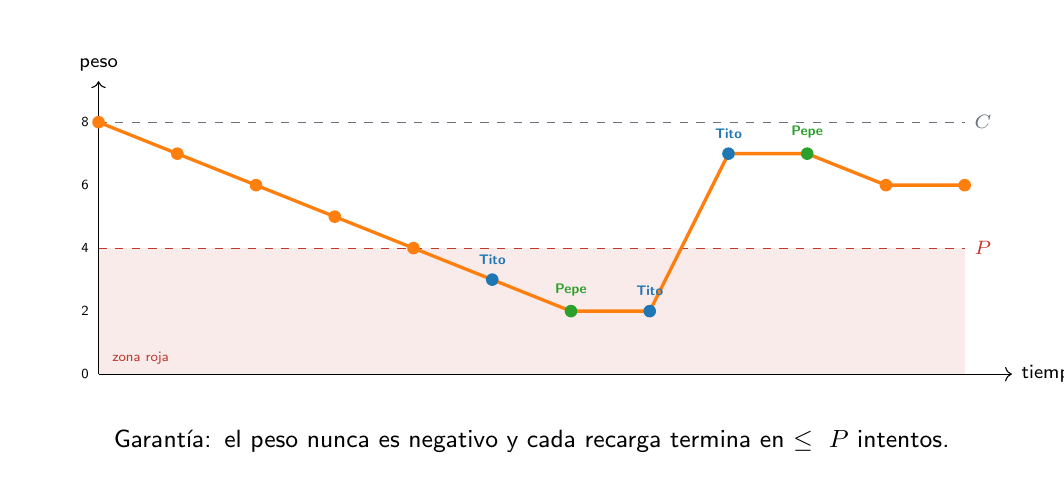
\begin{tikzpicture}
\useasboundingbox[fill=white] (0,0) rectangle (12.8,5.6);
\fill[acento!10] (0.9,1.2) rectangle (11.9,2.8);
\node[font=\tiny, acento, anchor=south west] at (0.95,1.2) {zona roja};
\draw[dashed, acento] (0.9,2.8) -- (11.9,2.8) node[right, font=\scriptsize] {$P$};
\draw[dashed, gris] (0.9,4.4) -- (11.9,4.4) node[right, font=\scriptsize] {$C$};
\draw[->] (0.9,1.2) -- (0.9,4.920000000000001) node[above, font=\scriptsize] {peso};
\draw[->] (0.9,1.2) -- (12.5,1.2) node[right, font=\scriptsize] {tiempo};
\node[left, font=\tiny] at (0.9,1.2) {0};
\node[left, font=\tiny] at (0.9,2.0) {2};
\node[left, font=\tiny] at (0.9,2.8) {4};
\node[left, font=\tiny] at (0.9,3.6000000000000005) {6};
\node[left, font=\tiny] at (0.9,4.4) {8};
\draw[very thick, cFol] (0.9,4.4) -- (1.9,4.0) -- (2.9,3.6000000000000005) -- (3.9,3.2) -- (4.9,2.8) -- (5.9,2.4000000000000004) -- (6.9,2.0) -- (7.9,2.0) -- (8.9,4.0) -- (9.9,4.0) -- (10.9,3.6000000000000005) -- (11.9,3.6000000000000005);
\fill[cFol] (0.9,4.4) circle (0.08);
\fill[cFol] (1.9,4.0) circle (0.08);
\fill[cFol] (2.9,3.6000000000000005) circle (0.08);
\fill[cFol] (3.9,3.2) circle (0.08);
\fill[cFol] (4.9,2.8) circle (0.08);
\fill[cLib] (5.9,2.4000000000000004) circle (0.08);
\node[font=\tiny\bfseries, text=cLib, above=2pt] at (5.9,2.4000000000000004) {Tito};
\fill[cWil] (6.9,2.0) circle (0.08);
\node[font=\tiny\bfseries, text=cWil, above=2pt] at (6.9,2.0) {Pepe};
\fill[cLib] (7.9,2.0) circle (0.08);
\node[font=\tiny\bfseries, text=cLib, above=2pt] at (7.9,2.0) {Tito};
\fill[cLib] (8.9,4.0) circle (0.08);
\node[font=\tiny\bfseries, text=cLib, above=2pt] at (8.9,4.0) {Tito};
\fill[cWil] (9.9,4.0) circle (0.08);
\node[font=\tiny\bfseries, text=cWil, above=2pt] at (9.9,4.0) {Pepe};
\fill[cFol] (10.9,3.6000000000000005) circle (0.08);
\fill[cFol] (11.9,3.6000000000000005) circle (0.08);
\node[font=\small, text width=12.2cm, align=center, text=black] at (6.4,0.35) {Garantía: el peso nunca es negativo y cada recarga termina en $\le P$ intentos.};
\end{tikzpicture}
\end{document}
